% Reporte del modelo generalizable de rendimiento municipal. Mismo formato que docs/reporte_regimenes.
% Compilar desde docs/reporte_generalizable (dos veces, para las referencias cruzadas):
%   xelatex -interaction=nonstopmode main.tex && xelatex -interaction=nonstopmode main.tex
% Las figuras y las cifras salen de scripts/figuras.py (ver el encabezado de ese archivo).
\documentclass[conference,letterpaper]{IEEEtran}
\usepackage{fontspec}
\setmainfont{TeX Gyre Termes}
\usepackage{polyglossia}
\setdefaultlanguage{spanish}
\usepackage{amsmath,amssymb}
\usepackage{graphicx}
\usepackage{booktabs}
\usepackage{array}
\usepackage{xcolor}
\usepackage{tikz}
\usetikzlibrary{positioning,arrows.meta}
\usepackage{hyperref}
\hypersetup{colorlinks=true,linkcolor=black,citecolor=black,urlcolor=blue!50!black}
\graphicspath{{figuras/}}

\newcommand{\code}[1]{\texttt{#1}}
\newcommand{\si}{\textcolor{green!45!black}{sí}}
\newcommand{\no}{\textcolor{red!70!black}{no}}

% ---------------------------------------------------------------- datos de la portada
\newcommand{\universidad}{Benemérita Universidad Autónoma de Puebla}
\newcommand{\facultad}{Facultad de Ciencias de la Computación}
\newcommand{\carrera}{Reto AgroCebada FIRA 2026}
\newcommand{\materia}{Reporte del modelo generalizable}
\newcommand{\integranteA}{José Alán Pomares Valdés}
\newcommand{\integranteB}{Luis Emmanuel Ramiro Luna}
\newcommand{\integranteC}{Vicente Josimar López Martinez}
\newcommand{\correo}{pv202351433@alm.buap.mx}
\newcommand{\asesor}{Ivan Olmos Pineda}
\newcommand{\fecha}{9 de octubre de 2026}

\newcommand{\logo}[2]{%
  \IfFileExists{figuras/#1}{\includegraphics[height=2.4cm]{#1}}%
  {\fbox{\parbox[c][2.2cm][c]{2.2cm}{\centering\footnotesize\textcolor{gray}{#2}}}}}

\begin{document}

% ---------------------------------------------------------------- portada
\begin{titlepage}
  \centering
  \begin{tabular}{@{}m{2.6cm}@{}m{\dimexpr\textwidth-5.2cm}@{}m{2.6cm}@{}}
    \logo{logo_buap.png}{Logo BUAP} &
    \centering{\Large\bfseries \universidad}\\[4pt]{\large \facultad} &
    \hfill\logo{logo_fcc.png}{Logo FCC}
  \end{tabular}\par
  \vspace{4pt}\rule{\textwidth}{1.2pt}\par
  \vspace{1.2cm}
  {\large \carrera}\par\vspace{4pt}
  {\large \materia}\par
  \vspace{3cm}
  {\Huge\bfseries ¿Dónde rinde más la\\[6pt] cebada de temporal?}\par
  \vspace{0.8cm}
  {\Large Un modelo municipal con datos públicos para\\[4pt] Hidalgo, México, Puebla y Tlaxcala}\par
  \vfill
  \begin{tabular}{@{}r@{\hspace{1em}}l@{}}
    \textbf{Integrantes} & \integranteA \\
                         & \integranteB \\
                         & \integranteC \\[4pt]
    \textbf{Asesor}      & \asesor \\[4pt]
    \textbf{Contacto}    & \href{mailto:\correo}{\correo} \\
  \end{tabular}\par
  \vspace{1.5cm}
  {\large Puebla, Pue., \fecha}\par
\end{titlepage}

\noindent\textbf{\textit{Resumen.}} \bfseries Estimamos el rendimiento esperado de la cebada de temporal en cada
municipio de Hidalgo, México, Puebla y Tlaxcala, y su probabilidad de quedar bajo 2\,t/ha, con datos públicos. La
etiqueta es el rendimiento oficial del SIAP de 2003 a 2025, que aplica el mismo criterio a todos los municipios. Comparamos
interpoladores espaciales con modelos ambientales simples fijados de antemano, con validación espacial y zonas de
exclusión de 0 a 80\,km. Sin datos a menos de 50\,km, la temperatura máxima de julio y agosto predice el nivel
municipal mejor que el kriging de los vecinos, con un error de 0.490 contra 0.566\,t/ha. El modelo final suma el kriging
de sus residuos y baja el error a 0.438\,t/ha. Con vecinos cerca la ventaja es pequeña y depende de cómo se pondere. El
suelo no agrega información detectable y el clima mensual del año no pronostica la cosecha. Publicamos una capa de 268
municipios con intervalo de 80\,\% y una marca de confianza.\par\mdseries

\smallskip
\noindent\textbf{\textit{Palabras clave.}} \bfseries cebada de temporal, rendimiento municipal, SIAP, validación
espacial, kriging, riesgo agrícola.\par\mdseries

\section{Introducción}\label{sec:intro}

FIRA financia y asegura siembras de cebada de temporal, la que depende solo de la lluvia. Hidalgo, Tlaxcala y Puebla
están entre los cinco estados con mayor producción nacional de cebada grano~\cite{sader2025}. FIRA necesita saber qué
rendimiento esperar, y con qué riesgo, en lugares donde no hay parcelas medidas.

Las etiquetas del reto no sirven para eso. Se dividen por municipio en dos grupos que promedian 4.49 y 3.05\,t/ha.
Los rendimientos de un grupo se registran con dos decimales y los del otro están redondeados. Un reporte técnico
interno del equipo~\cite{regimenes} probó clima, altitud, suelo, fenología por satélite y cercanía al Popocatépetl,
y ninguna de esas variables explica la diferencia de 1.44\,t/ha entre los grupos. Por eso usamos el rendimiento
oficial del Servicio de Información Agroalimentaria y Pesquera (SIAP)~\cite{siap}. El SIAP publica una cifra por
municipio con el mismo procedimiento de reporte. Eso no asegura que se haya medido igual en campo, y el SIAP a veces
copia una misma cifra entre municipios (Sección~\ref{sec:datos}). El modelo predice el rendimiento promedio de un
municipio según esa cifra oficial, no el de una parcela.

\textbf{Resultados principales.}
\begin{itemize}
\item \textbf{La cebada rinde más donde el verano es fresco.} Cada grado más de temperatura máxima en julio y agosto
se asocia con cerca de 0.8\,t/ha menos. Es una asociación y no prueba que el calor sea la causa.
\item \textbf{Ese dato basta para estimar lugares sin datos.} Lejos de municipios con SIAP, el modelo de temperatura
se equivoca menos que copiar a los vecinos, 0.44 contra 0.57\,t/ha. Como elegimos la variable viendo resultados, una
selección repetida dentro de la validación reduce la ventaja de 0.13 a cerca de 0.07\,t/ha.
\item \textbf{El suelo y el clima del año no ayudan.} El suelo no mejora el modelo y el clima mensual del año no
anticipa la cosecha.
\end{itemize}

\section{Datos}\label{sec:datos}

\textbf{Rendimiento.} Usamos el cierre agrícola municipal del SIAP para cebada grano de temporal en
primavera-verano, de 2003 a 2025~\cite{siap}. Quitamos las cosechas de menos de 50\,ha y los municipios con menos de
5 años de datos. Quedan 1\,942 registros municipio-año de 100 municipios, unos 25 por estado.

\textbf{Unidad de análisis.} La unidad es el municipio. Para cada uno promediamos sus años con una media simple. Cada
municipio tiene entre 5 y 23 años, con mediana de 22. El modelo se ajusta y se evalúa con esos 100 promedios. Los
1\,942 registros no son observaciones independientes, porque los de un mismo municipio se parecen entre sí.

\textbf{Tendencia.} El rendimiento sube en promedio 0.028\,t/ha por año, estimado con los 100 municipios. Esa cifra es
descriptiva. Con ella llevamos cada año al nivel de 2025 antes de promediar, para dibujar los mapas y las
dispersiones. En la validación la pendiente se estima de nuevo en cada partición, solo con los municipios de
entrenamiento, y se suma a la predicción de cada año. Entre particiones con zona de exclusión de 50\,km la pendiente
es inestable y va de 0.013 a 0.050\,t/ha por año. Sin tendencia el RMSE del modelo final sería 0.417\,t/ha en lugar de
0.438. Es decir que la tendencia no mejora la métrica, porque esta compara promedios de todos los años de cada
municipio. El nivel de 2025 tampoco se valida con esa métrica. Con solo los 76 registros de 2025, el error por
registro del modelo final es de 0.88\,t/ha.

\textbf{Cifras repetidas.} El SIAP muchas veces estima una cifra por distrito y la copia a varios municipios. En 1\,036
de los 1\,942 registros (53\,\%) la cifra coincide, a dos decimales, con la de otro municipio del mismo estado y año.
En total, 651 pares de municipios comparten una cifra idéntica en al menos un año. La zona de exclusión de 50\,km
no impide que una cifra repetida quede en el entrenamiento y en la prueba. Con esa zona, 154 de los 651 pares
quedan separados entre ambos conjuntos, y el 10.7\,\% de los registros de prueba conserva un gemelo en el
entrenamiento (38.9\,\% sin zona de exclusión). Al quitar del entrenamiento esos gemelos, el RMSE sube entre 0.001
y 0.005\,t/ha y el orden de los modelos no cambia.

\textbf{Ambiente.} Usamos lluvia de CHIRPS~\cite{chirps}, temperatura máxima (Tmax) y mínima de
CHIRTS-ERA5~\cite{chirts,verdin2020,hersbach2020}, elevación y pendiente del Copernicus DEM~\cite{copdem} y la carta
de suelos del INEGI~\cite{inegi_eda}. Cada variable se promedia solo sobre la agricultura de temporal del
municipio~\cite{inegi_usv}, en los 486 municipios del Marco Geoestadístico~\cite{inegi_mg}.

La Fig.~\ref{fig:mapas_obs} muestra el patrón central. Los municipios con mejor rendimiento están donde el verano es
más fresco, en el oriente de Puebla, Tlaxcala y el centro del Estado de México.

\begin{figure*}[t]
\centering
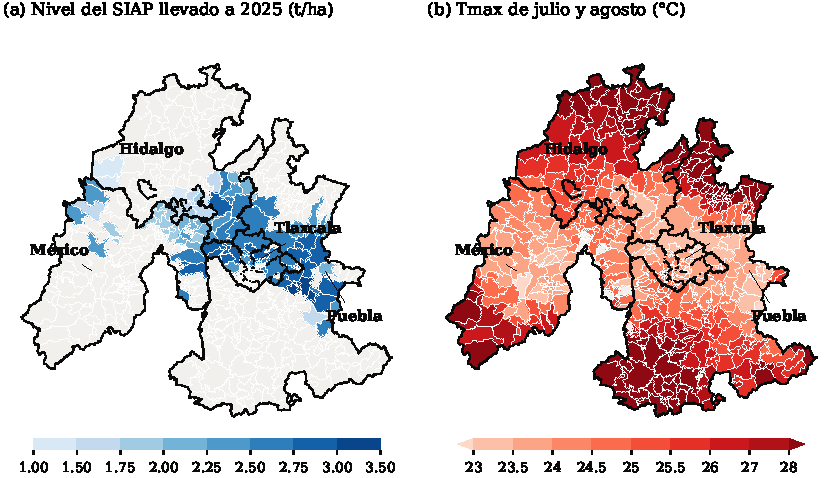
\includegraphics[width=\textwidth]{g_mapas_obs}
\caption{(a) Rendimiento oficial promedio de cada municipio con datos del SIAP, llevado a 2025. (b) Temperatura
máxima promedio de julio y agosto en la agricultura de temporal de cada municipio.}
\label{fig:mapas_obs}
\end{figure*}

\section{Método}\label{sec:metodo}

\textbf{Modelos.} Comparamos dos formas de estimar el rendimiento promedio de un municipio.
\begin{itemize}
\item \textbf{Kriging de vecinos.} Estima un municipio con un promedio ponderado del rendimiento de los municipios
con SIAP, donde los más próximos pesan más. Los pesos no se fijan a mano. Se aprenden de los datos midiendo qué tanto
se parecen los rendimientos de dos municipios según la distancia que los separa~\cite{rasmussen2006,oliver2014}. Es la
base a superar porque no usa ambiente.
\item \textbf{Modelos ambientales simples.} Regresiones lineales con una o dos variables elegidas por lo que se sabe
del cultivo. La principal usa la Tmax de julio y agosto, porque en la cebada unos pocos días de calor sobre la espiga
durante el llenado reducen el peso del grano~\cite{passarella2002}.
\end{itemize}
También probamos modelos con 14 variables de clima, terreno y suelo.

\textbf{Detalle del kriging.} Es un proceso gaussiano sobre las coordenadas de los centroides municipales. La
covarianza entre dos municipios a distancia $d$ es una Matérn de suavidad $\nu = 3/2$ más ruido blanco,
\[
k(d) = \sigma^2\Bigl(1 + \tfrac{\sqrt{3}\,d}{\ell}\Bigr)e^{-\sqrt{3}\,d/\ell} + \tau^2\,\mathbf{1}[d = 0].
\]
El ruido $\tau^2$ representa el error propio del promedio de cada municipio. La longitud de correlación $\ell$ y las
varianzas $\sigma^2$ y $\tau^2$ se estiman por máxima verosimilitud en cada partición, solo con los municipios de
entrenamiento. La media es una constante igual al promedio de los promedios municipales. La optimización parte de
$\ell = 30$\,km con cotas de 2 a 500\,km, usa tres inicios y semilla fija. El ruido tiene una cota inferior, la mitad
de la mediana de la varianza de la media de cada municipio entre la varianza entre municipios. Con zona de exclusión
de 50\,km, $\ell$ promedia 35\,km (de 12.6 a 85.7), $\sigma^2 = 0.16$ y $\tau^2 = 0.05$ (t/ha)$^2$. En 24.5\,\% de las
particiones el ruido queda en su cota inferior, así que esa cota condiciona el resultado cuando hay pocos municipios.

\textbf{Tmax.} Es la temperatura máxima diaria promedio de julio y agosto sobre la agricultura de temporal del
municipio, promediada de 2003 a 2025. Sale de CHIRTS-ERA5~\cite{chirts,verdin2020} y no del SIAP, así que existe para
cualquier municipio, tenga o no datos de rendimiento. Los rendimientos del SIAP solo sirven para ajustar la
regresión, es decir, para saber cuánto cambia el rendimiento por cada grado de Tmax.

\textbf{Modelo final.} Combina los dos anteriores en dos pasos. Primero la regresión con Tmax da un rendimiento para
cada municipio. Después calculamos su error en cada municipio con SIAP, la diferencia entre el rendimiento observado y
el predicho, y aplicamos el kriging a esos errores en lugar de al rendimiento. Si los vecinos de un municipio rinden
más de lo que su Tmax predice, por manejo, variedad o suelo, el municipio recibe parte de esa corrección. Lejos de
municipios con SIAP la corrección se acerca a cero y queda solo la predicción por Tmax. El kriging de estos errores se
ajusta igual que el anterior. Su longitud de correlación baja a unos 14\,km y su ruido a 0.014\,(t/ha)$^2$, porque
tras quitar la Tmax queda una correlación espacial muy local. Su ruido toca la cota inferior en 34\,\% de las
particiones con zona de exclusión.

\textbf{Validación.} Agrupamos los 100 municipios en 20 zonas con el método de k-medias sobre sus coordenadas y
predecimos una zona a la vez sin usar sus datos. Una validación espacial evita que la autocorrelación infle el
desempeño~\cite{roberts2017,ploton2020}. Para simular un lugar realmente nuevo quitamos además los municipios a menos
de $B = 50$\,km de la zona (Fig.~\ref{fig:validacion}). Con $B = 0$ solo se deja fuera la zona. Repetimos todo 10
veces con agrupamientos distintos. Las repeticiones comparten los mismos 100 municipios, así que no son pruebas
independientes. Para medir la incertidumbre remuestreamos los municipios 4\,000 veces (bootstrap) y reportamos
intervalos de 95\,\%.

\textbf{Error.} Usamos la raíz del error cuadrático medio (RMSE) en t/ha entre el rendimiento promedio predicho
$\bar p_i$ y el observado $\bar y_i$ de cada municipio $i$,
\[
\mathrm{RMSE} = \sqrt{\frac{\sum_i w_i\,(\bar p_i - \bar y_i)^2}{\sum_i w_i}}.
\]
El peso $w_i$ es la superficie sembrada media del municipio, en forma lineal. Va de 50 a 21\,136\,ha, con mediana de
687\,ha. Los 10 municipios con más superficie suman el 51\,\% del peso y el tamaño efectivo de muestra
$1/\sum_i (w_i/\sum_j w_j)^2$ es 28 de 100. Ponderamos porque FIRA opera donde hay más superficie. Las regresiones se
ajustan con mínimos cuadrados con los mismos pesos y el kriging no usa pesos. También reportamos el RMSE sin pesos
entrenando sin pesos las regresiones, para que la comparación sea justa.

\textbf{Regla de decisión.} La fijamos antes de correr los experimentos. Un modelo ambiental sustituye al kriging si gana
en al menos 7 de las 10 repeticiones y si su ventaja desaparece al revolver las variables entre municipios.

\begin{figure}[!tbp]
\centering
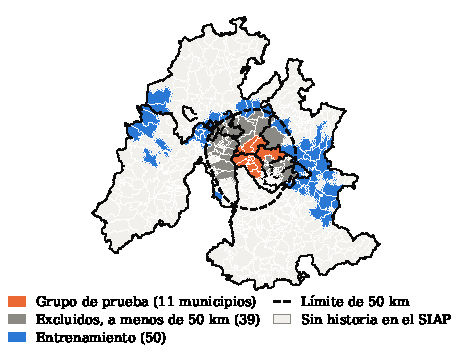
\includegraphics[width=\columnwidth]{g_validacion}
\caption{Una partición de la validación. El modelo se entrena sin los municipios grises y predice los naranjas, como
si fueran un lugar sin datos del SIAP a menos de 50\,km.}
\label{fig:validacion}
\end{figure}

\section{Resultados}\label{sec:resultados}

\subsection{Comparación de modelos}

La Tabla~\ref{tab:modelos} reúne el RMSE de nivel de cada modelo en los escenarios de validación, y la
Fig.~\ref{fig:exclusion} muestra cómo crece con la zona de exclusión.

\begin{table*}[t]
\centering
\caption{RMSE de nivel municipal (t/ha), media de 10 repeticiones. Pond. indica ponderado por superficie sembrada.
En negritas, el menor de cada columna. n.d. indica que el modelo no se evaluó en ese escenario.}
\label{tab:modelos}
\footnotesize
\begin{tabular}{@{}lcccccc@{}}
\toprule
 & \multicolumn{2}{c}{$B = 0$\,km} & \multicolumn{2}{c}{$B = 50$\,km} & Por distrito & Sin repetidos, $B = 0$ \\
\cmidrule(lr){2-3}\cmidrule(lr){4-5}
Modelo & Pond. & Sin ponderar & Pond. & Sin ponderar & Pond. & Pond. \\
\midrule
Media global & 0.504 & 0.488 & 0.594 & 0.579 & 0.534 & 0.592 \\
Media estatal & 0.451 & 0.410 & 0.644 & 0.530 & 0.497 & 0.532 \\
IDW de vecinos & 0.349 & 0.349 & 0.560 & 0.510 & 0.446 & 0.402 \\
Kriging de vecinos & 0.309 & \textbf{0.343} & 0.566 & 0.518 & 0.503 & 0.402 \\\midrule
Tmax jul-ago & 0.334 & 0.457 & 0.490 & 0.511 & 0.373 & 0.422 \\
Elevación & 0.437 & 0.509 & 0.631 & 0.623 & 0.481 & 0.546 \\
Tmax y lluvia & 0.272 & 0.426 & 0.506 & 0.515 & \textbf{0.305} & \textbf{0.365} \\
Tmax, lluvia y dúrica & 0.287 & 0.434 & 0.592 & 0.575 & 0.334 & 0.374 \\
Tmax y lluvia con estado & 0.305 & 0.426 & 0.541 & 0.546 & 0.494 & 0.380 \\\midrule
Tmax con kriging de residuos (final) & 0.293 & 0.411 & \textbf{0.438} & \textbf{0.459} & 0.393 & 0.383 \\
Tmax y lluvia con kriging de residuos & \textbf{0.269} & 0.427 & 0.464 & 0.496 & 0.359 & 0.369 \\\midrule
Ridge, 14 variables & 0.302 & 0.469 & 0.662 & 0.617 & 0.354 & n.d. \\
Lasso, 14 variables & 0.302 & 0.460 & 0.612 & 0.585 & 0.332 & n.d. \\
\bottomrule
\end{tabular}
\end{table*}

\begin{figure}[t]
\centering
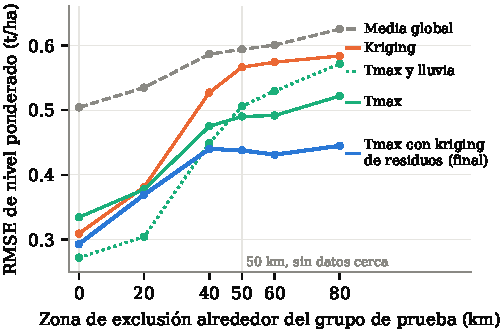
\includegraphics[width=\columnwidth]{g2_exclusion}
\caption{RMSE de nivel ponderado contra el radio de la zona de exclusión. A mayor radio, más lejos queda el municipio
de prueba del SIAP de entrenamiento más cercano.}
\label{fig:exclusion}
\end{figure}

\begin{itemize}
\item \textbf{Sin datos cerca, el ambiente supera al kriging.} Con $B = 50$\,km el kriging de vecinos tiene un RMSE
ponderado de 0.566\,t/ha. El modelo de Tmax de julio y agosto baja a 0.490 y gana en 10 de 10 repeticiones con
$p = 0.01$. El de Tmax y lluvia baja a 0.506, también con 10 de 10 y $p = 0.01$. Con el kriging de los residuos de
Tmax el error queda en 0.438 y gana en 10 de 10, ponderado y sin ponderar. Con 80\,km queda en 0.445, contra 0.584 del
kriging.
\item \textbf{Con vecinos cerca, la ventaja depende de la ponderación.} Con $B = 0$ y ponderando, el modelo de Tmax y
lluvia tiene 0.272 contra 0.309 del kriging, con 10 de 10 y $p = 0.01$. El kriging de residuos de Tmax tiene 0.293,
con 7 de 10 y $p = 0.02$. Sin ponderar, el kriging gana a todos los modelos ambientales en las 10 repeticiones, con
0.343 contra 0.411 del kriging de residuos de Tmax. Los municipios chicos tienen medias ruidosas que se parecen a las
de sus vecinos, y el clima no las explica. En los municipios con al menos 1\,000\,ha sembradas el kriging de
residuos de Tmax tiene 0.274 contra 0.307 del kriging.
\item \textbf{Por distrito, el kriging pierde su ventaja.} Al dejar fuera un DDR completo, el kriging sube a
0.503\,t/ha, cerca de la media global (0.534). El modelo de Tmax y lluvia queda en 0.305 y el kriging de residuos de
Tmax en 0.393. Parte de la ventaja del kriging venía de que el SIAP copia la cifra dentro del distrito.
\item \textbf{Sin cifras repetidas, el orden se mantiene.} Con las 862 filas sin repetir y $B = 0$, el kriging tiene
0.402, el kriging de residuos de Tmax 0.383 y el modelo de Tmax y lluvia 0.365.
\item \textbf{Más variables no ayudan.} El ridge y el lasso de 14 variables quedan cerca del kriging con $B = 0$
(0.302 ambos, contra 0.309) y le ganan solo en 4 de 10 repeticiones. Además se degradan con la distancia. Con $B = 50$\,km tienen 0.662 y 0.612, peor que la media global (0.594). La
elevación sola tampoco basta (0.631).
\end{itemize}

\textbf{Modelo final.} Por la regla fijada, el modelo de Tmax pasa contra el kriging con $B = 50$\,km. Entre las
variantes que la pasan elegimos la de menor promedio de la métrica principal en 0 y 50\,km, que es el kriging de los
residuos de Tmax, con 0.366\,t/ha. El kriging de vecinos promedia 0.438 y el modelo de Tmax solo 0.412. Lejos de los
datos se comporta como el modelo de clima y cerca corrige con el SIAP observado.

\subsection{Qué variables importan}

La Fig.~\ref{fig:importancia} muestra la importancia condicional y marginal de cada bloque.

\begin{figure}[t]
\centering
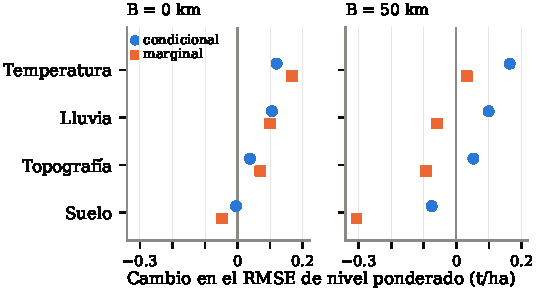
\includegraphics[width=\columnwidth]{g3_importancia}
\caption{Importancia por bloque con 99 permutaciones. Condicional, cuánto empeora el modelo de cuatro bloques al
revolver el bloque. Marginal, cuánto mejora un modelo con solo el bloque sobre la media global. Valores positivos
indican que el bloque ayuda.}
\label{fig:importancia}
\end{figure}

\begin{itemize}
\item \textbf{La temperatura es el bloque más fuerte.} Con $B = 0$, revolverla empeora el modelo en 0.120\,t/ha y sola
mejora a la media global en 0.167, ambas con $p = 0.01$. Con $B = 50$\,km es el único bloque que mejora por sí solo,
en 0.032 con $p = 0.01$.
\item \textbf{La lluvia agrega información propia.} Con $B = 0$ su importancia condicional es 0.106 y la marginal
0.100, ambas con $p = 0.01$.
\item \textbf{La topografía explica algo, pero casi todo lo comparte con la temperatura.} Sola mejora 0.070
($p = 0.01$), pero dado el resto agrega solo 0.038 ($p = 0.02$). La elevación y la Tmax de julio y agosto tienen una
correlación de $-0.80$ entre municipios.
\item \textbf{El suelo no agrega información detectable.} Con $B = 0$ su importancia condicional es $-0.005$
($p = 0.64$) y solo empeora a la media global en 0.049 ($p = 0.90$).
\item \textbf{Más bloques extrapolan mal.} Con $B = 50$\,km el modelo de cuatro bloques tiene 0.607\,t/ha, peor que la
media global (0.594).
\end{itemize}

La relación con la temperatura es fuerte y sencilla. Ajustado con todos los datos, el modelo de Tmax predice
0.79\,t/ha menos por cada grado más de Tmax media en julio y agosto. Con la lluvia en el modelo, el efecto es de
0.67\,t/ha por grado y la lluvia suma 0.15\,t/ha por cada 100\,mm entre mayo y octubre. Entre los municipios con SIAP
la Tmax de julio y agosto va de 23.0 a 25.7\,$^\circ$C y su correlación con el nivel es $-0.60$. Es una asociación
entre municipios, no un efecto causal.

\subsection{El clima del año no pronostica la cosecha}

Las anomalías del año parecen útiles en la validación espacial, pero no por el clima. La Fig.~\ref{fig:clima_anio}
compara el RMSE por municipio y año.

\begin{figure}[t]
\centering
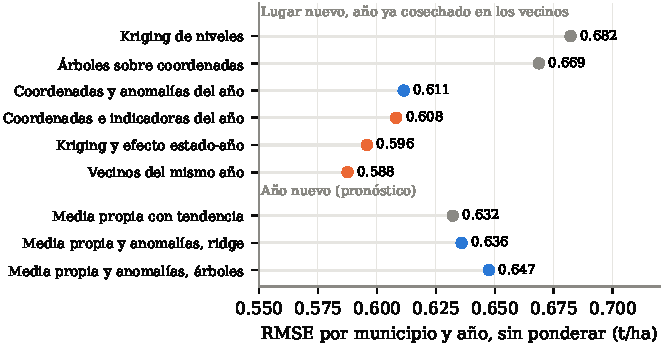
\includegraphics[width=\columnwidth]{g4_clima_anio}
\caption{RMSE por municipio y año sin ponderar. Arriba, validación espacial, donde los municipios de entrenamiento
ya traen la cosecha del mismo año. Abajo, validación por año. En azul, los modelos con anomalías de clima. En
naranja, los que usan la cosecha del año sin clima.}
\label{fig:clima_anio}
\end{figure}

\begin{itemize}
\item \textbf{En la validación espacial, las anomalías equivalen a indicadoras de año.} Un modelo de árboles de
gradiente sobre las coordenadas tiene 0.669\,t/ha. Con las anomalías baja a 0.611 y gana en 10 de 10 repeticiones.
Pero con indicadoras de año en lugar de anomalías baja a 0.608, y las anomalías solo le ganan en 3 de 10. Una
indicadora de año es una variable que vale uno en ese año y cero en los demás. Las anomalías son casi iguales en toda
la región, así que el modelo las usa para reconocer el año y copiar la cosecha de los vecinos. El kriging con el
efecto del estado en el año (0.596) y los vecinos del mismo año (0.588) hacen lo mismo sin clima.
\item \textbf{En la validación por año, las anomalías no mejoran.} La media propia de cada municipio con tendencia
tiene 0.632\,t/ha. Agregar las anomalías da 0.636 con ridge y 0.647 con árboles. Ponderando, la media propia tiene
0.603 y con anomalías y ridge 0.602, un empate. Con clima mensual no se puede pronosticar un año nuevo.
\end{itemize}

\subsection{Riesgo y cobertura}

Con la escala global, Puebla quedó con una cobertura de 0.740 con $B = 0$, debajo del mínimo de 0.75. La escala local
la sube a 0.819, así que la regla eligió la escala local.
\begin{itemize}
\item \textbf{Con datos cerca la cobertura es cercana a la nominal.} Con $B = 0$ es 0.815 sin ponderar y 0.825
ponderada. Por estado va de 0.778 en Hidalgo a 0.859 en Tlaxcala. El ancho medio del intervalo es 1.862\,t/ha.
\item \textbf{Sin datos cerca el intervalo se ensancha.} Con $B = 50$\,km la cobertura es 0.815 sin ponderar y 0.797
ponderada, con un ancho medio de 2.060\,t/ha. Hidalgo subcubre, con 0.740.
\item \textbf{La probabilidad bajo 2\,t/ha sobreestima un poco el riesgo.} Con $B = 0$ la probabilidad media es 0.475 y
la fracción observada de años bajo 2\,t/ha es 0.411. El puntaje de Brier, el error cuadrático medio de la
probabilidad, es 0.199.
\item \textbf{El rendimiento sobre sembrada se cubre igual.} Su cobertura con $B = 0$ es 0.817.
\end{itemize}

\subsection{Capa municipal}

Aplicamos el modelo final a los 486 municipios de los cuatro estados (Fig.~\ref{fig:mapas}). Solo publicamos valores
en los 268 municipios cuyo ambiente cae dentro del rango de los municipios con SIAP. Los otros 218 son sobre todo
tierras bajas y calientes donde no se siembra cebada de temporal y donde el modelo lineal extrapola. Cada municipio
con valor lleva una marca de confianza.
\begin{itemize}
\item \textbf{Alta.} El municipio tiene historia propia en el SIAP. Son 100.
\item \textbf{Media.} Sin historia propia, pero con agricultura de temporal, a no más de 25\,km de un municipio con
SIAP y dentro del dominio. El dominio pide además al menos 100\,ha de temporal y SIAP a no más de 50\,km. Son 91.
\item \textbf{Baja.} El resto de los municipios con valor. Son 77.
\end{itemize}

\begin{figure*}[t]
\centering
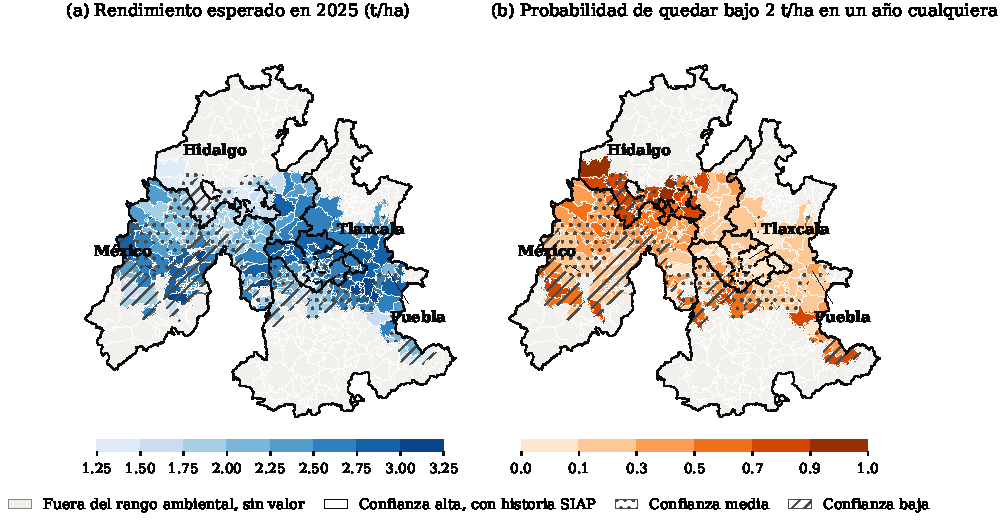
\includegraphics[width=\textwidth]{g5_mapas}
\caption{Rendimiento oficial esperado en 2025 y probabilidad de quedar bajo 2\,t/ha en un año cualquiera, por
municipio. El rayado marca la confianza media (puntos) y baja (líneas). En gris claro, los municipios fuera del rango
ambiental de los municipios con SIAP, sin valor.}
\label{fig:mapas}
\end{figure*}

\begin{itemize}
\item \textbf{El rendimiento esperado va de 1.26 a 3.16\,t/ha.} La mediana de los municipios de confianza alta es
2.53\,t/ha, con una probabilidad mediana de 0.23 de quedar bajo 2\,t/ha. El ancho mediano del intervalo es
1.90\,t/ha.
\item \textbf{Los mejores municipios con historia están en el oriente de Puebla.} San Salvador el Seco y San Juan
Atenco esperan 3.16\,t/ha, con probabilidad de 0.18 de quedar bajo 2\,t/ha.
\item \textbf{Los peores están en Hidalgo.} Huichapan espera 1.33\,t/ha, San Agustín Tlaxiaca 1.38 y Nopala de
Villagrán 1.43, con probabilidades de 0.91, 0.99 y 0.88.
\item \textbf{La marca de confianza separa a los municipios frescos sin tradición cebadera.} De los 10 municipios con
mayor rendimiento esperado, 5 son de confianza alta, 2 de media y 3 de baja. Jilotzingo (3.08\,t/ha) y Huixquilucan
(2.97) quedan en baja porque están a 37 y 47\,km del municipio con SIAP más cercano. Tlalmanalco (3.07) queda en
media porque está a 18\,km de uno, aunque solo tiene 237\,ha de temporal.
\end{itemize}

\subsection{Relación con las etiquetas del reto}

Para los 9 municipios del reto predijimos su nivel en 2025 sin usarlos en el ajuste y lo comparamos con la media de
sus parcelas por régimen (Fig.~\ref{fig:reto}). La comparación es descriptiva.

\begin{figure}[t]
\centering
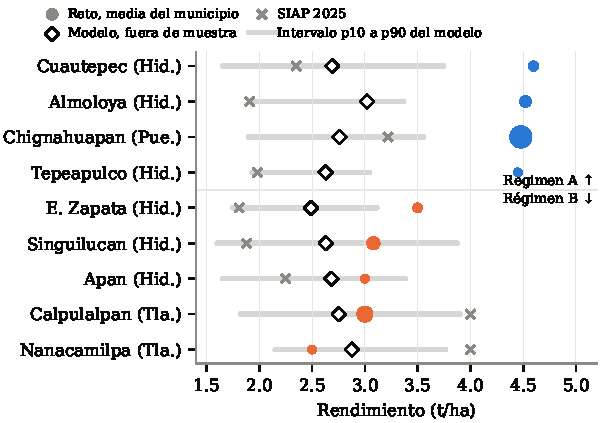
\includegraphics[width=\columnwidth]{g6_reto}
\caption{Media de las parcelas del reto por municipio (círculos, tamaño según el número de parcelas), nivel del
modelo fuera de muestra con su intervalo p10 a p90 y rendimiento del SIAP en 2025.}
\label{fig:reto}
\end{figure}

\begin{itemize}
\item \textbf{El régimen A queda muy arriba del modelo.} Sus 87 parcelas en 4 municipios promedian 4.49\,t/ha y el
modelo da 2.78, una diferencia de 1.71\,t/ha. Por municipio va de 1.50 a 1.91. El SIAP de 2025 de esos municipios
promedia 3.01.
\item \textbf{El régimen B se parece al modelo.} Sus 51 parcelas en 5 municipios promedian 3.05\,t/ha y el modelo da
2.70, una diferencia de 0.35. Por municipio va de $-0.38$ a 1.01. El SIAP de 2025 promedia 3.17.
\end{itemize}
Esto es consistente con que las etiquetas del régimen A miden otra cosa que el promedio municipal, pero no lo prueba.

\section{Limitaciones}\label{sec:discusion}

\begin{itemize}
\item \textbf{El modelo aprende la cifra que publica el SIAP.} Esa cifra a veces se estima por distrito y se copia
entre municipios, y puede diferir de lo que obtiene un productor. La zona de exclusión no impide que una cifra
repetida quede en el entrenamiento y en la prueba, aunque quitarlas cambia el error en menos de 0.005\,t/ha.
\item \textbf{Pocas unidades independientes.} El modelo usa 100 promedios municipales, y 10 de ellos concentran la
mitad del peso en el error. Las 10 repeticiones comparten esos municipios, así que los intervalos por remuestreo
son más fiables que el conteo de repeticiones ganadas.
\item \textbf{Asociación, no causa.} La temperatura también refleja la altura, la tradición cebadera y el manejo. El
modelo ordena lugares, pero no dice cuánto cambiaría el rendimiento si cambiara el clima.
\item \textbf{La elección de Tmax sola se hizo viendo resultados.} El contendiente fijado de antemano era Tmax con
lluvia, que queda casi empatado y es mejor con vecinos cerca. La selección anidada reduce la ventaja sobre el
kriging de 0.13 a cerca de 0.07\,t/ha. Como trabajo futuro, la prueba más limpia es validar el modelo con datos del
SIAP de otros estados productores de cebada, que ni los datos ni la elección de variables hayan visto.
\item \textbf{Los intervalos y las probabilidades son aproximados.} La cobertura de 81.5\,\% es marginal y baja a
64.7\,\% en 2025. La probabilidad no está calibrada, y por eso la presentamos solo como apoyo preliminar.
\item \textbf{Municipios frescos sin cebada.} Un municipio fresco puede salir alto aunque ahí no se siembre cebada o
su suelo sea forestal. Por eso lleva confianza baja.
\end{itemize}

\section{Conclusiones y uso para crédito y seguro}\label{sec:conclusiones}

Construimos un modelo del rendimiento municipal de la cebada de temporal con datos públicos y lo validamos como si
cada municipio fuera un lugar nuevo. La temperatura máxima de julio y agosto, corregida con el kriging de los
residuos, predice el nivel municipal con un RMSE ponderado de 0.293\,t/ha con datos cerca y de 0.438\,t/ha sin datos a
menos de 50\,km. El kriging de vecinos tiene 0.309 y 0.566. El suelo no agrega información detectable y el clima
mensual del año no pronostica la cosecha.

Para FIRA proponemos tres usos.
\begin{enumerate}
\item \textbf{Priorizar zonas para crédito.} El rendimiento esperado y su intervalo p10 a p90 ordenan los municipios
por su potencial. Los de confianza alta tienen una mediana de 2.53\,t/ha. Los de confianza media sirven para ampliar
la cobertura a municipios vecinos sin historia propia.
\item \textbf{Tarifar el seguro.} La probabilidad de quedar bajo 2\,t/ha en un año cualquiera resume el riesgo de cada
municipio. Entre los municipios de confianza alta va de 0.00 en Lázaro Cárdenas, Tlaxcala, a 0.99 en San
Agustín Tlaxiaca, Hidalgo. Como sobreestima un poco la
frecuencia observada, es una cota prudente. Para el seguro conviene usar el rendimiento sobre sembrada, que incluye la
pérdida por siniestro.
\item \textbf{Exigir verificación donde la confianza es baja.} En los 77 municipios de confianza baja el valor solo
refleja el clima. Antes de financiar ahí hace falta confirmar que se siembra cebada y que el suelo es agrícola.
\end{enumerate}

El modelo predice el promedio de un municipio. El rendimiento de un productor depende además de su manejo, y las
etiquetas del régimen A del reto quedan 1.71\,t/ha arriba del modelo. Para estimar el rendimiento de una parcela
harán falta datos de manejo y rendimientos medidos con un mismo criterio en todos los municipios.


% Sólo las referencias citadas en el texto, en estilo IEEE y en orden de aparición.
\begin{thebibliography}{10}

\bibitem{regimenes}
J.~A. Pomares Valdés, L.~E. Ramiro Luna y V.~J. López Martinez, ``¿Qué separa a los dos regímenes de rendimiento?
Descarte de causas ambientales y contraste con las cifras oficiales del SIAP,'' reporte técnico, Reto AgroCebada
FIRA 2026, Facultad de Ciencias de la Computación, BUAP, Puebla, 2026.

\bibitem{siap}
Servicio de Información Agroalimentaria y Pesquera, ``Cierre de la producción agrícola por municipio, cebada grano,
temporal, primavera-verano, 2003--2025.'' [En línea]. Disponible: \url{https://nube.agricultura.gob.mx/cierre_agricola/}.
Consultado el 9 de octubre de 2026.

\bibitem{chirps}
C.~Funk \emph{et al.}, ``The climate hazards infrared precipitation with stations, a new environmental record for
monitoring extremes,'' \emph{Scientific Data}, vol.~2, art.~150066, 2015.

\bibitem{chirts}
Climate Hazards Center, Universidad de California en Santa Bárbara, ``CHIRTS-ERA5, temperatura máxima y mínima
mensual.'' [En línea]. Disponible: \url{https://data.chc.ucsb.edu/experimental/CHIRTS-ERA5/}. Consultado el 9 de
octubre de 2026.

\bibitem{copdem}
Agencia Espacial Europea, ``Copernicus DEM GLO-90.'' [En línea]. Disponible:
\url{https://copernicus-dem-90m.s3.amazonaws.com/}. Consultado el 9 de octubre de 2026.

\bibitem{inegi_eda}
Instituto Nacional de Estadística y Geografía, ``Conjunto de datos vectorial edafológico, escala 1:250\,000, Series I
y II.'' [En línea]. Disponible: \url{https://www.inegi.org.mx/temas/edafologia/}

\bibitem{inegi_usv}
Instituto Nacional de Estadística y Geografía, ``Conjunto de datos vectoriales de uso del suelo y vegetación, escala
1:250\,000, Serie VII, conjunto nacional,'' 2021. [En línea]. Disponible: \url{https://www.inegi.org.mx/temas/usosuelo/}

\bibitem{inegi_mg}
Instituto Nacional de Estadística y Geografía, ``Marco Geoestadístico 2025.'' [En línea]. Disponible:
\url{https://www.inegi.org.mx/app/biblioteca/ficha.html?upc=794551163061}

\bibitem{roberts2017}
D.~R. Roberts \emph{et al.}, ``Cross-validation strategies for data with temporal, spatial, hierarchical, or
phylogenetic structure,'' \emph{Ecography}, vol.~40, no.~8, pp.~913--929, 2017.

\bibitem{angelopoulos2023}
A.~N. Angelopoulos y S.~Bates, ``Conformal prediction, a gentle introduction,'' \emph{Foundations and Trends in
Machine Learning}, vol.~16, no.~4, pp.~494--591, 2023.

\end{thebibliography}

\end{document}
